\documentclass[tikz,border=0pt]{standalone}
\usepackage[american]{circuitikz}
\usetikzlibrary{arrows.meta,calc,positioning,decorations.pathmorphing,patterns}
\definecolor{zyloTeal}{HTML}{174A5B}
\definecolor{zyloTealTwo}{HTML}{246B7A}
\definecolor{zyloInk}{HTML}{1F2933}
\definecolor{zyloSoft}{HTML}{EAF4F4}
\definecolor{zyloPaper}{HTML}{F8FAFB}
\definecolor{zyloLine}{HTML}{44606B}
\definecolor{zyloOrange}{HTML}{D97706}
\begin{document}
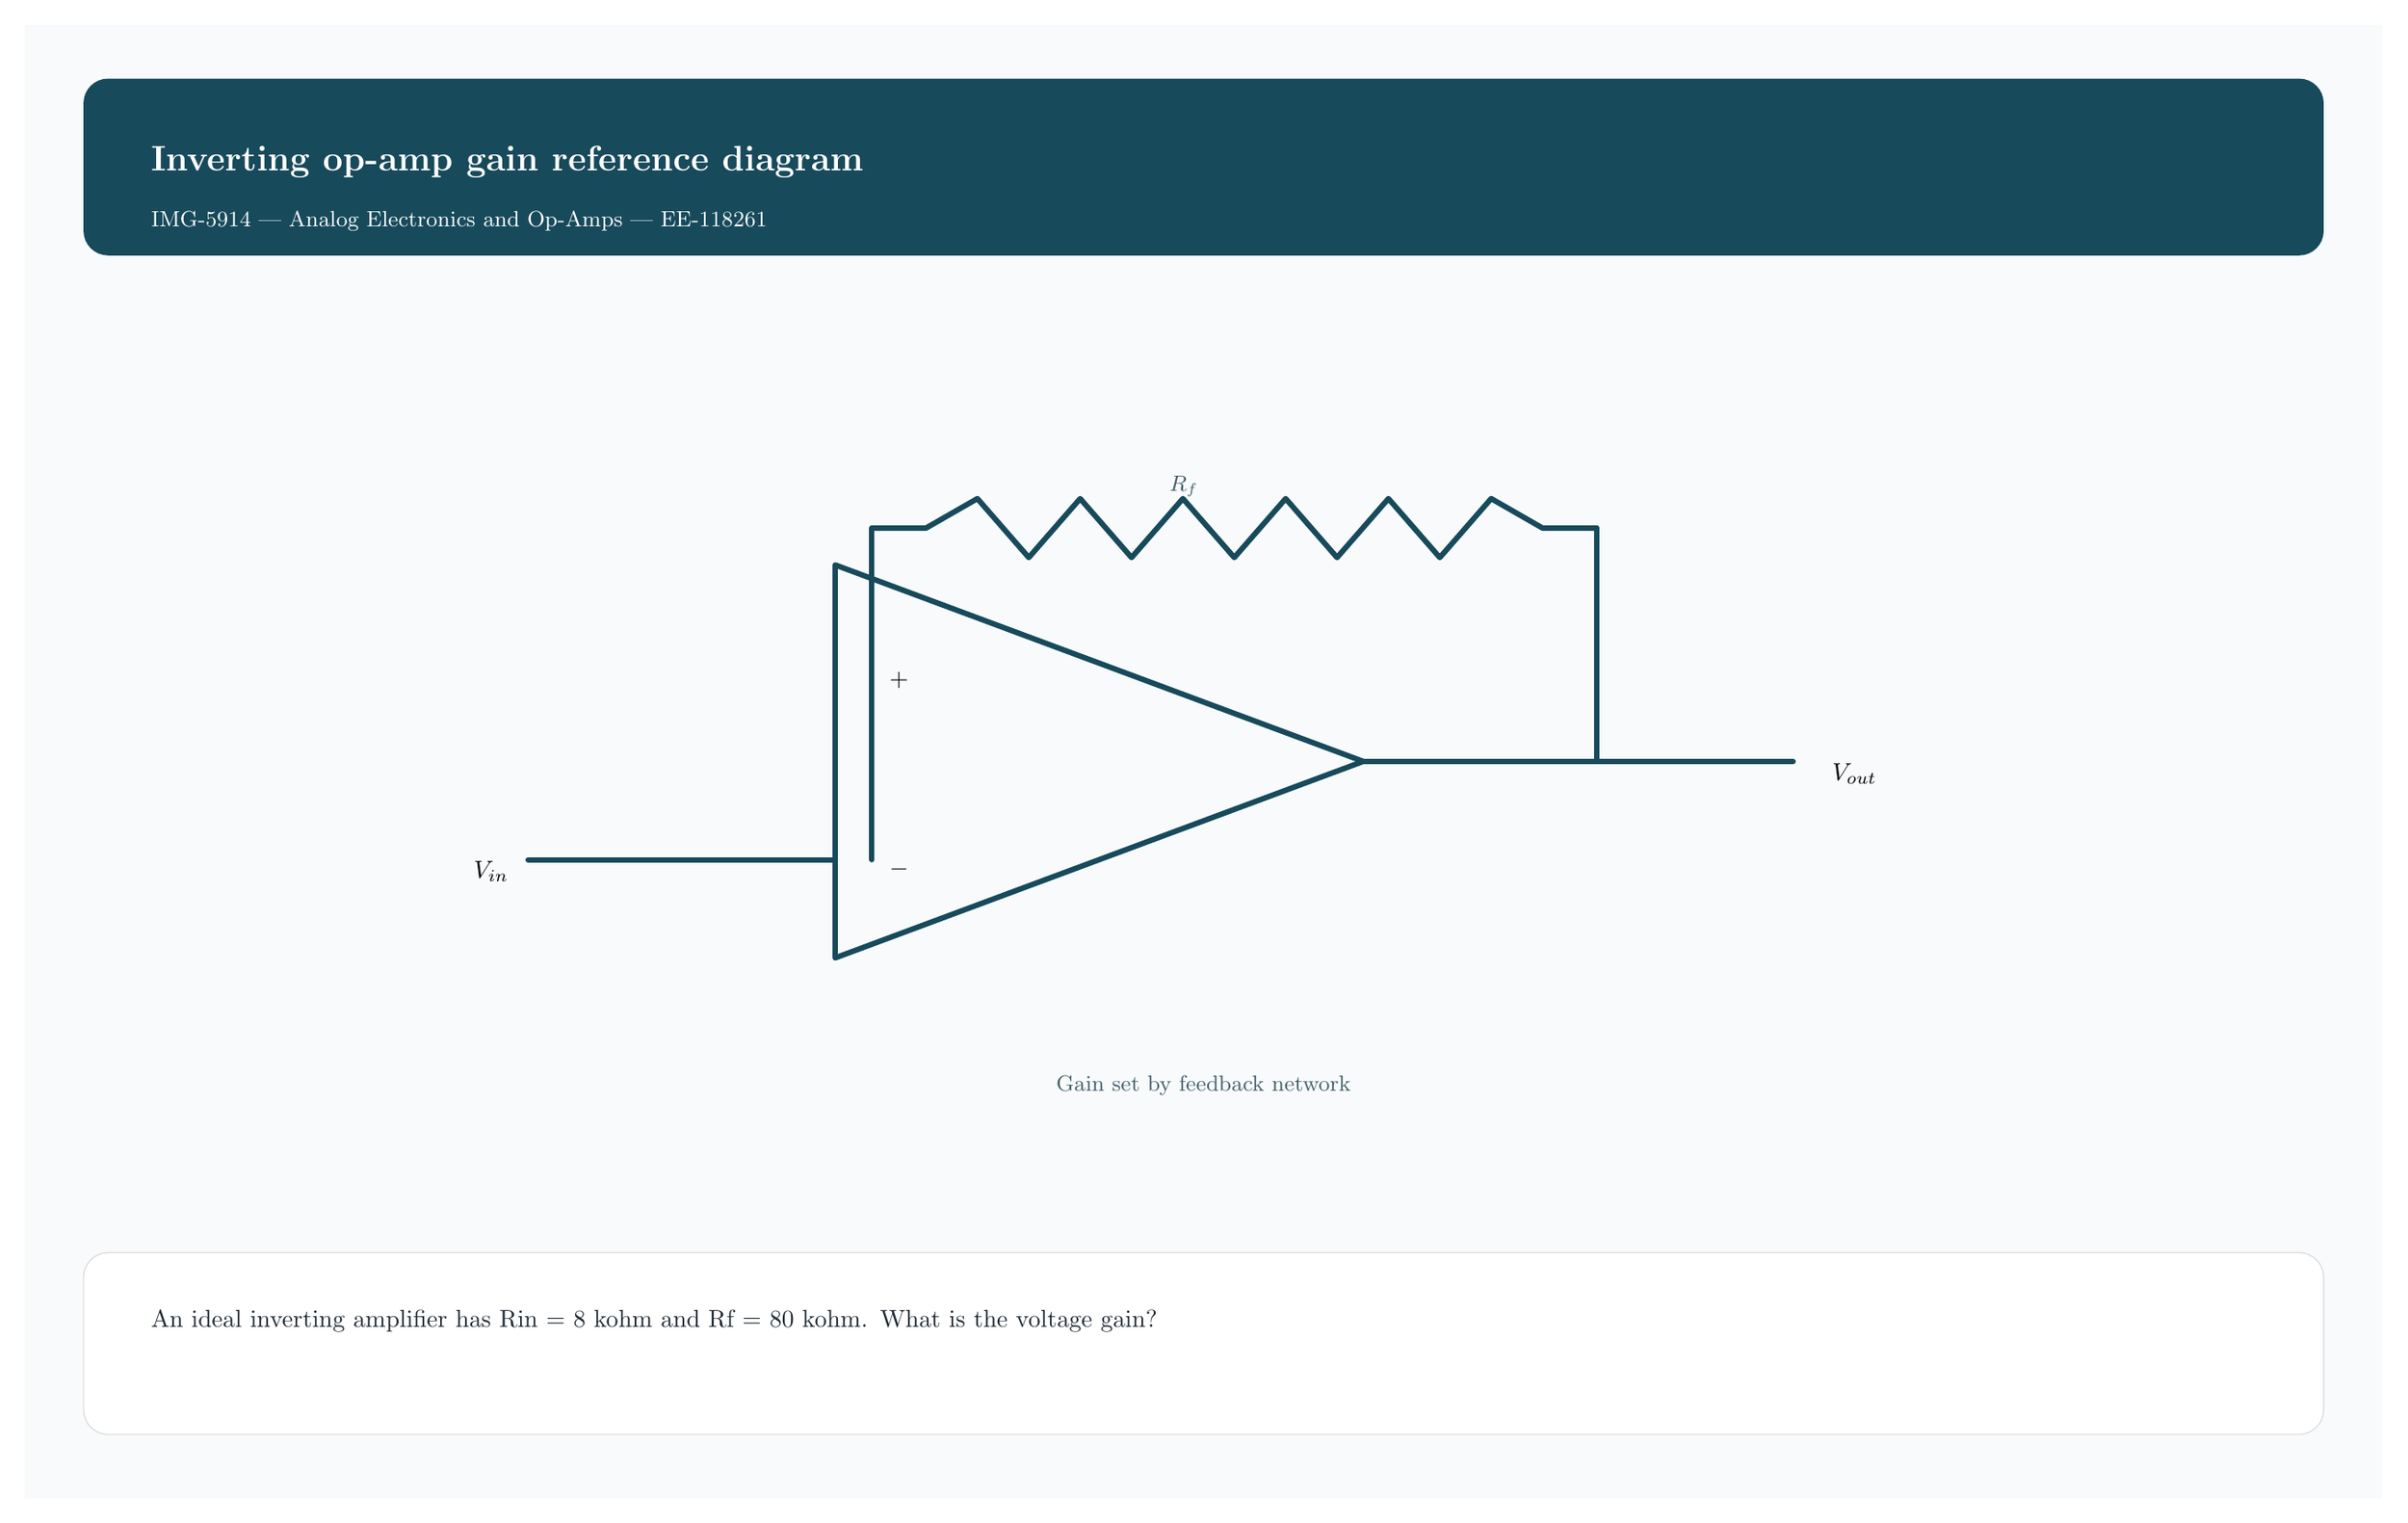
\begin{tikzpicture}[x=1pt,y=-1pt,>=Latex,line cap=round,line join=round]
\path[fill=zyloPaper] (0,0) rectangle (960,600);
\path[fill=zyloTeal,rounded corners=10pt] (24,22) rectangle (936,94);
\node[anchor=west,text=white,font=\bfseries\Large] at (48,56) {Inverting op-amp gain reference diagram};
\node[anchor=west,text=white!82,font=\small] at (48,80) {IMG-5914 | Analog Electronics and Op-Amps | EE-118261};
\tikzset{wire/.style={draw=zyloTeal,line width=2.2pt},thinwire/.style={draw=zyloLine,line width=1.35pt},accent/.style={draw=zyloOrange,line width=2.2pt},box/.style={draw=zyloTealTwo,fill=zyloSoft,line width=1.5pt,rounded corners=8pt}}
\draw[wire] (330,220) -- (330,380) -- (545,300) -- cycle;
\node at (356,267) {$+$}; \node at (356,344) {$-$};
\draw[wire] (205,340) -- (330,340);
\draw[wire] (545,300) -- (720,300);
\draw[wire] (345,205) -- (367,205) -- (367,205) -- (387.917,193) -- (408.833,217) -- (429.75,193) -- (450.667,217) -- (471.583,193) -- (492.5,217) -- (513.417,193) -- (534.333,217) -- (555.25,193) -- (576.167,217) -- (597.083,193) -- (618,205) -- (640,205);
\draw[wire] (345,205) -- (345,340); \draw[wire] (640,205) -- (640,300);
\node[font=\small,text=zyloLine] at (472,188) {$R_f$}; \node at (190,345) {$V_{in}$}; \node at (745,305) {$V_{out}$};
\node[font=\small,text=zyloLine] at (480,432) {Gain set by feedback network};
\path[draw=black!15,fill=white,rounded corners=10pt] (24,500) rectangle (936,574);
\node[anchor=west,text width=860pt,align=left,text=zyloInk,font=\normalsize] at (48,528) {An ideal inverting amplifier has Rin = 8 kohm and Rf = 80 kohm. What is the voltage gain?};
\end{tikzpicture}
\end{document}
